\section{Introduction}\label{sec:introduction}

Planetary exploration aims to provide scientific insights to advance our knowledge about other planets, their geology and available resources. Analysis of samples plays a key role in this endeavor, where extraterrestrial robotic systems are instrumental in their acquisition for either in-situ analysis or sample return~\cite{zhang_progress_2019}. Reports of these findings are also necessary for future in-situ resource utilization~\cite{moses_frontier_2016} to enable extraction of Hydrogen and Oxygen for localized production of rocket propellant and operation of life support systems. In this way, the required payload during the initial launch from Earth would be significantly reduced while decreasing the dependency on additional resupply missions. There is an increasing effort put into sample return missions that could provide this data. Lunar material was recently returned to Earth by the Chang'e~5 mission~\cite{liu_landing_2021}, and NASA has selected companies to collect Moon rocks towards the progress of the Artemis program~\cite{schierholz_nasa_2020}. Mars Sample Return is another proposed mission, where an ESA rover is planned to fetch samples that are being collected by the NASA rover Perseverance~\cite{muirhead_mars_2019}. Unfortunately, communication delay causes remote teleoperation to be inefficient, which reduces the amount of scientific data that rovers can gather throughout their mission. Therefore, autonomy for extraterrestrial rovers becomes essential as the complexity of missions increases.

\begin{figure}[t]
	\vspace{2.057mm}
	\centering
	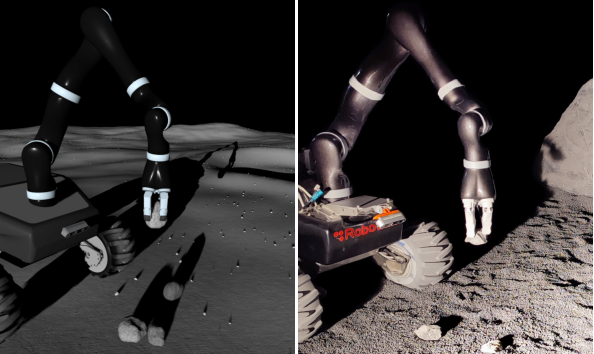
\includegraphics[width=1.0\linewidth]{title_image.pdf}
	\caption{Our agents learn vision-based robotic grasping under challenging conditions in a heavily randomized simulation environment. Their performance is then evaluated on a real robot inside a Moon-analogue facility.}
	\label{fig:front_page_figure}
	\vspace{-1.0\baselineskip}
\end{figure}

Rovers equipped with robotic arms have many potential applications in extraterrestrial environments. Besides manipulating science instruments to closely analyze areas of interest, these rovers could also perform assembly and maintenance tasks by interacting with various tools and technical equipment. Many subroutines involved in such tasks require an object or a tool to be firmly grasped prior to performing them. Therefore, robotic grasping is a fundamental skill that is essential for flexible mobile manipulation. In order to achieve this flexibility, rovers are required to grasp a diversity of objects that can differ in their geometry, appearance and mechanical properties.

We present an approach for applying end-to-end deep reinforcement learning to the task of vision-based robotic grasping in lunar environments. The primary focus of this paper is to learn end-to-end policies for robotic grasping under challenging conditions of the Moon, i.e.~unstructured scenes with uneven terrain, diverse rocks and harsh illumination. As the training of agents directly in extraterrestrial conditions is unfeasible due to the high cost and safety requirements of space robotic systems, our goal is to employ simulations with the aim of transferring learned policies to a real robot.

The main contributions of this work are as follows:
\begin{itemize}
	\item A simulation environment of the Moon, which enables learning of mobile manipulation skills that are transferable to the real-world domain due to its realistic physics, physically-based rendering and extensive use of domain randomization with procedurally-generated datasets for simulating the wide variety of lunar conditions.
	\item A novel approach for utilizing 3D octree visual observations with multi-channel features for end-to-end deep reinforcement learning. Octrees are used to efficiently represent the 3D scene, while an octree-based convolutional neural network is applied to extract abstract features that allow agents to generalize over spatial positions and orientations.
	\item A demonstration of learning robotic grasping inside a realistic simulation environment of the Moon and subsequent zero-shot sim-to-real transfer to a real robot inside a Moon-analogue facility.
\end{itemize}
